
\documentclass{article}
\usepackage{natbib}
\usepackage[utf8]{inputenc}
\usepackage{geometry}
 \geometry{
 a4paper,
 total={170mm,257mm},
 left=20mm,
 top=20mm,
 }
 \usepackage{graphicx}
 \usepackage{subcaption}
 \usepackage{titling}
 \usepackage{float}
 \usepackage{amsmath}
\usepackage{listings}
\usepackage{color}
\usepackage{tikz}
\usepackage{graphicx}
\usepackage{caption}
\usepackage{subcaption}
\usepackage{tikz}
\usepackage{pgfplots}
\usetikzlibrary{spy,calc}
\usepackage{hyperref}

 \title{ASSIGNMENT 2: Computer Vision 792}
\author{Madhia Shabih}
\date{August 2024}
 
 \usepackage{fancyhdr}
\fancypagestyle{plain}{%  the preset of fancyhdr 
    \fancyhf{} % clear all header and footer fields
    \fancyfoot[L]{\thedate}
    \fancyhead[L]{24397644}
    \fancyhead[R]{\theauthor}
}
\makeatletter
\def\@maketitle{%
  \newpage
  \null
  \vskip 1em%
  \begin{center}%
  \let \footnote \thanks
    {\LARGE \@title \par}%
    \vskip 1em%
    %{\large \@date}%
  \end{center}%
  \par
  \vskip 1em}
\makeatother

\usepackage{lipsum}  
\usepackage{cmbright}

\title{Computer Vision Report: Camera Matrix and Epipolar Geometry}
\author{Madhia Shabih}
\date{\today}

\begin{document}
\maketitle

\section{Problem 1: Computing a Camera Matrix}

\subsection{1a: World Coordinate System and Camera Matrix Calculation}
\textbf{Description:} \\
% Explain how you chose the world coordinate axes and identified at least 28 corner points on the object in "lego1.jpg". 
% Describe the method used to determine the 2D image coordinates and 3D world coordinates. Include a table of correspondences if necessary.
Figure \ref{fig:lego1} below describes how I chose the world coordinate axes and Table 1 below includes the table of correspondences which I 
determined. I calculated the 2D image coordinates by selecting 28 corners of the legos. I then converted it to 3D world coordinates,
allowing the intersection on the X-, Y- and Z- coordinate to be (0, 0, 0) and then incrementing the respective amount in mm to the point where 
I had selected a corner.

\begin{table}[H]
    \centering
    \begin{tabular}{|c|c|c|c|c|c|}
    \hline
    \textbf{x} & \textbf{y} & \textbf{x'} & \textbf{y'} & \textbf{z'} \\
    \hline
    1547 & 1840 & 0   & 0   & 0     \\
    1557 & 1267 & 0   & 0   & 67.2  \\
    1562 & 937  & 0   & 0   & 105.6 \\
    1073 & 1749 & 0   & 64  & 0     \\
    404  & 1606 & 0   & 160 & 0     \\
    1873 & 1659 & 80  & 0   & 0     \\
    2328 & 1418 & 208 & 0   & 0     \\
    1430 & 1494 & 16  & 0   & 38.4  \\
    732  & 1372 & 0   & 112 & 38.4  \\
    961  & 1097 & 0   & 80  & 76.8  \\
    302  & 985  & 0   & 176 & 76.8  \\
    1320 & 901  & 0   & 32  & 105.6 \\
    849  & 827  & 0   & 96  & 105.6 \\
    409  & 771  & 0   & 160 & 105.6 \\
    1188 & 1611 & 0   & 48  & 19.2  \\
    737  & 1530 & 0   & 112 & 19.2  \\
    305  & 1443 & 0   & 176 & 19.2  \\
    1746 & 1661 & 48  & 0   & 0     \\
    1993 & 1536 & 112 & 0   & 0     \\
    2219 & 1419 & 176 & 0   & 0     \\
    2430 & 1302 & 240 & 0   & 0     \\
    1819 & 1233 & 64  & 0   & 57.6  \\
    2066 & 1129 & 128 & 0   & 57.6  \\
    2283 & 1020 & 192 & 0   & 57.6  \\
    2026 & 684  & 112 & 0   & 124.8 \\
    2357 & 561  & 208 & 0   & 124.8 \\
    852  & 745  & 0   & 96  & 124.8 \\
    198  & 653  & 0   & 192 & 124.8 \\
    \hline
    \end{tabular}
    \caption{2D Image Coordinates in Pixels and Corresponding 3D World Coordinates in mm}
    \end{table}

    \begin{figure}[H] % The [H] option places the figure exactly here
      \centering
      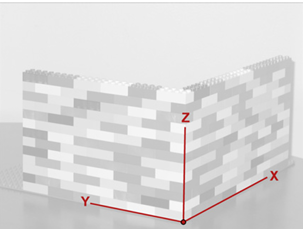
\includegraphics[width=0.3\textwidth]{axis.png} % Adjust the width as needed
      \caption{3D world co-ordinate system}
      \label{fig:lego1}
  \end{figure}

\textbf{Results:} \\
% Present the calculated camera matrix \(P\). Use the formula and explain briefly.
Below is the calculated P matrix: 

\subsection*{Homography Matrix \( P \)}
\[
P =
\begin{bmatrix}
2.75416038 \times 10^{-3} & -2.87589499 \times 10^{-3} & 5.85201094 \times 10^{-6} & 6.39998608 \times 10^{-1} \\
-2.34030798 \times 10^{-4} & -3.53935397 \times 10^{-4} & -3.46138168 \times 10^{-3} & 7.68357719 \times 10^{-1} \\
4.74050139 \times 10^{-7} & 1.15244558 \times 10^{-7} & -5.01027097 \times 10^{-8} & 4.22797122 \times 10^{-4}
\end{bmatrix}
\]

\subsection{1b: Proof of Camera Matrix Decomposition}
\textbf{Description:} \\
% Outline the proof that the camera matrix decomposition algorithm returns \(K\), \(R\), and \(\tilde{C}\) such that \(K\) is upper-triangular, 
% \(R\) is orthogonal, and \(KR[I - \tilde{C}]\) equals \(P\).
The upper triangular matrix has all the elements below the diagonal as zero. As one can observe (see \ref{sec:1c}), this is the case with the intrinsic matrix \(K\). 
\newline

A square matrix with real numbers or elements is said to be an orthogonal matrix if its transpose is equal to its inverse matrix. 
The inverse and transpose of the rotation matrix \( R \) are: 

\[
R^{-1} = \begin{bmatrix}
  0.24363231 & -0.966366 & 0.08234101 \\
  -0.07937672 & -0.10448198 & -0.99135405 \\
  0.966614 & 0.23498992 & -0.10216215
  \end{bmatrix}
\]

\[
R^T = \begin{bmatrix}
  0.24363231 & -0.966366 & 0.08234101 \\
  -0.07937672 & -0.10448198 & -0.99135405 \\
  0.966614 & 0.23498992 & -0.10216215
  \end{bmatrix}
\]

As one can see, these are identical and hence \( R \) is orthogonal. \\



\textbf{Discussion:} \\
Comment on the extent of uniqueness in the decomposition and its importance.

\subsection{1c: Camera Matrix Decomposition for Lego 1}
\textbf{Results:} \\
% Show the decomposition of matrix \(P\) into \(K\), \(R\), and \(\tilde{C}\). Scale \(K\) such that its bottom-right entry is 1. Include the necessary calculations and matrices.
\subsection*{Intrinsic Matrix \( K_1 \)}
\[
K_1 =
\begin{bmatrix}
7.03606595 \times 10^3 & 1.55093658 \times 10^2 & 4.04916599 \times 10^3 \\
0 & 7.11020543 \times 10^3 & 9.01944958 \times 10^1 \\
0 & 0 & 1
\end{bmatrix}
\]

\subsection*{Rotation Matrix \( R_1 \)}
\label{sec:1c}
\[
R_1 =
\begin{bmatrix}
0.24363231 & -0.966366 & 0.08234101 \\
-0.07937672 & -0.10448198 & -0.99135405 \\
0.966614 & 0.23498992 & -0.10216215
\end{bmatrix}
\]

\subsection*{Camera Center \( C_1 \)}
\[
C_1 =
\begin{bmatrix}
-739.8902994 \\
-485.37784529 \\
321.63665888
\end{bmatrix}
\]

\textbf{Discussion:} \\
Discuss the significance of the decomposed components.

%%%%%%%%%%%%%%%%%%%%%%%%%%%%%%%%%%%%%%%%%%%%%%%%%%%%%%%%%%%%%%%%%%%%%%%%%%%%%%%%%%%%%%%%%%%
\newpage
\section{Problem 2: Computing a Second Camera Matrix}

\subsection{2a: Repeating the Calculations for Lego 2}
\textbf{Description:} \\

\begin{table}[h!]
    \centering
    \begin{tabular}{|c|c|c|c|c|}
    \hline
    \textbf{x} & \textbf{y} & \textbf{x} (3D) & \textbf{y} (3D) & \textbf{z} (3D) \\
    \hline
    240 & 1440 & 0 & 192 & 0 \\
    242 & 1308 & 0 & 192 & 19.2 \\
    240 & 1178 & 0 & 192 & 38.4 \\
    242 & 1045 & 0 & 192 & 57.6 \\
    245 & 905 & 0 & 192 & 76.8 \\
    245 & 786 & 0 & 192 & 96 \\
    250 & 577 & 0 & 192 & 124.8 \\
    988 & 1758 & 0 & 0 & 0 \\
    991 & 1623 & 0 & 0 & 19.2 \\
    988 & 1471 & 0 & 0 & 38.4 \\
    991 & 1320 & 0 & 0 & 57.6 \\
    993 & 1180 & 0 & 0 & 76.8 \\
    998 & 1028 & 0 & 0 & 96 \\
    998 & 799 & 0 & 0 & 124.8 \\
    2424 & 1506 & 240 & 0 & 0 \\
    2421 & 1366 & 240 & 0 & 19.2 \\
    2424 & 1236 & 240 & 0 & 38.4 \\
    2434 & 1109 & 240 & 0 & 57.6 \\
    2439 & 972 & 240 & 0 & 76.8 \\
    2439 & 837 & 240 & 0 & 96 \\
    2447 & 625 & 240 & 0 & 124.8 \\
    \hline
    \end{tabular}
    \caption{2D Image Coordinates in Pixels and Corresponding 3D World Coordinates in mm}
    \end{table}

\textbf{Results:} \\
% Present the new camera matrix and the distance between the two camera centers and the angle between their principal axes.

\subsection*{Homography Matrix \( P \)}
\[
P =
\begin{bmatrix}
-3.45737581 \times 10^{-3} & 1.84680728 \times 10^{-3} & -1.34003533 \times 10^{-5} & -4.87876478 \times 10^{-1} \\
2.22192346 \times 10^{-4} & 3.96427196 \times 10^{-4} & 3.84370894 \times 10^{-3} & -8.72895156 \times 10^{-1} \\
-2.06695621 \times 10^{-7} & -3.04302600 \times 10^{-7} & 4.29616113 \times 10^{-8} & -4.94925813 \times 10^{-4}
\end{bmatrix}
\]

\subsection*{Intrinsic Matrix \( K_2 \)}
\[
K_2 =
\begin{bmatrix}
1.05251026 \times 10^4 & -5.99949679 \times 10^1 & 1.10856424 \times 10^3 \\
0 & 1.04504974 \times 10^4 & -1.04111217 \times 10^1 \\
0 & 0 & 1
\end{bmatrix}
\]

\subsection*{Rotation Matrix \( R_2 \)}
\[
R_2 =
\begin{bmatrix}
-0.82783123 & 0.5608882 & -0.00999388 \\
0.05685095 & 0.10160475 & 0.9931991 \\
-0.55808908 & -0.82163307 & 0.11599862
\end{bmatrix}
\]

\subsection*{Camera Center \( C_2 \)}
\[
C_2 =
\begin{bmatrix}
-721.05444208 \\
-1082.93989766 \\
380.46969249
\end{bmatrix}
\]

\textbf{Discussion:} \\
Analyze the differences between the two matrices and what they imply about the relative camera positions.

\subsection{2b: 3D Plot of Camera Positions and World Points}
\textbf{Results:} \\
\begin{figure}[h]
  \centering
  \begin{minipage}{0.45\textwidth}
      \centering
      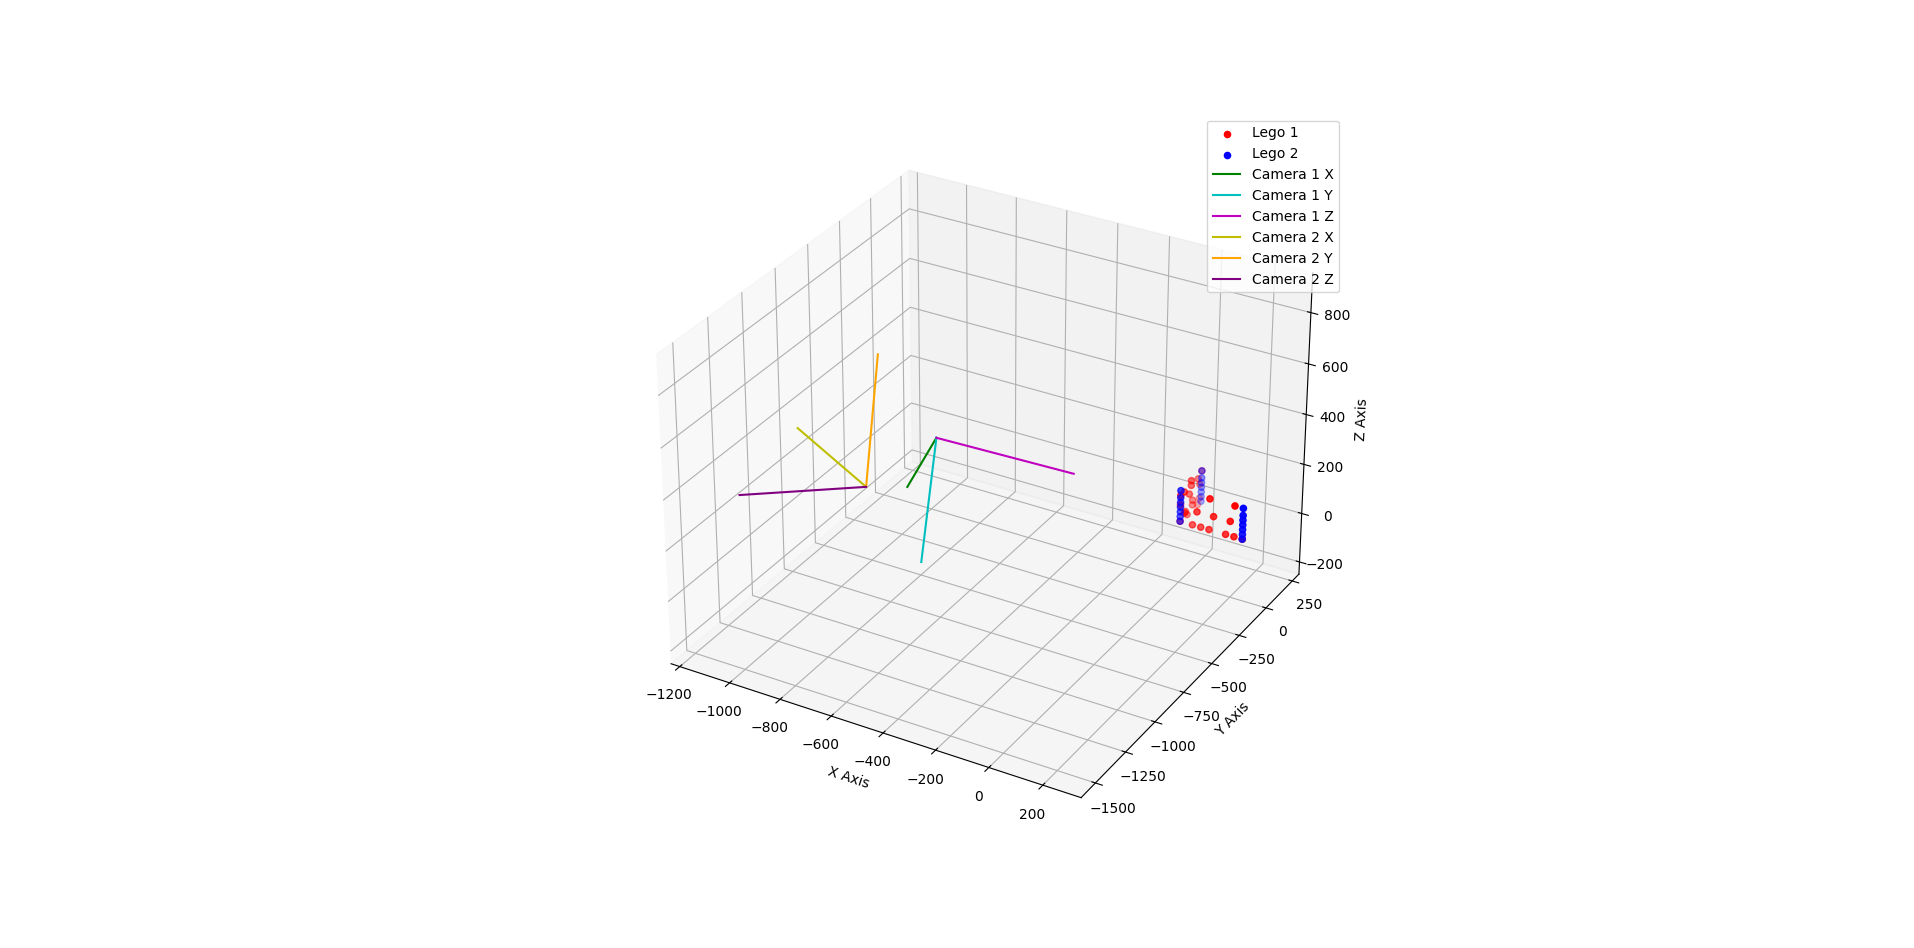
\includegraphics[width=\textwidth,  trim=350 0 350 0, clip]{Figure_1.png}
      \label{fig:image1}
  \end{minipage}\hfill
  \begin{minipage}{0.45\textwidth}
      \centering
      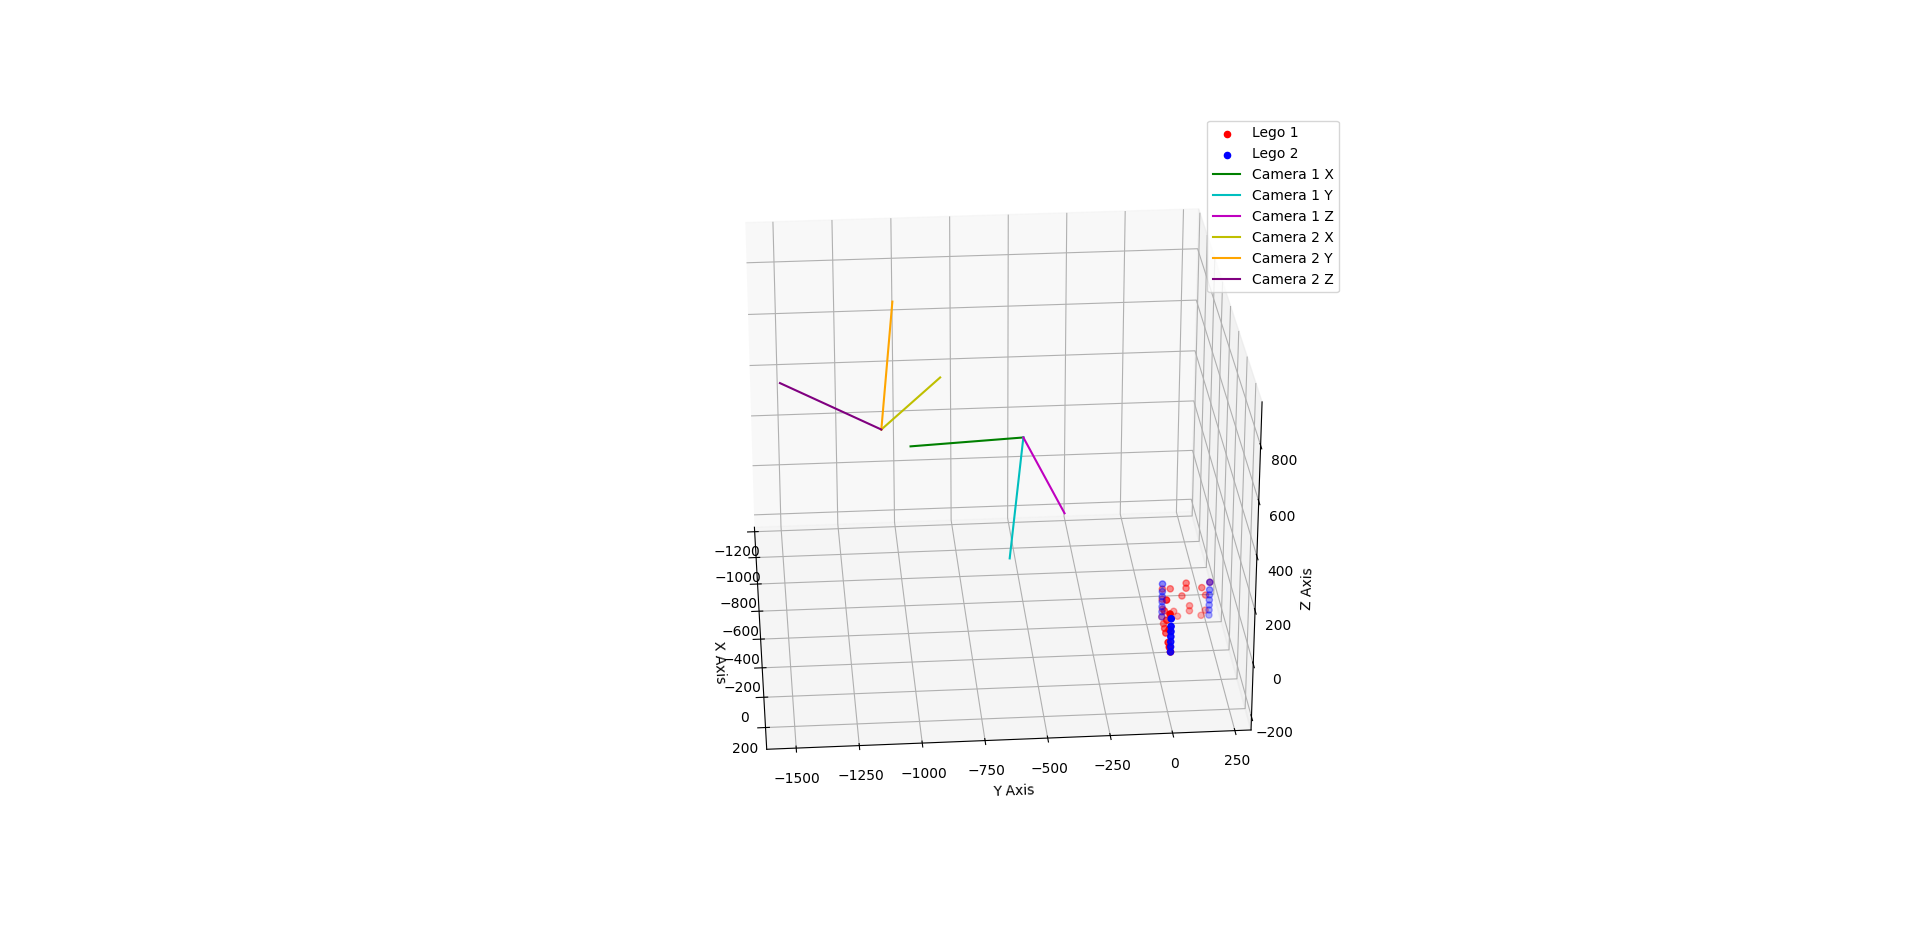
\includegraphics[width=\textwidth,  trim=350 0 350 0, clip]{Figure_2.png}
      \label{fig:image2}
  \end{minipage}
  \caption{Different views of 3D plot.}
  \label{fig:side_by_side}
\end{figure}
\begin{figure}[h]
  \centering
  \begin{minipage}{0.45\textwidth}
      \centering
      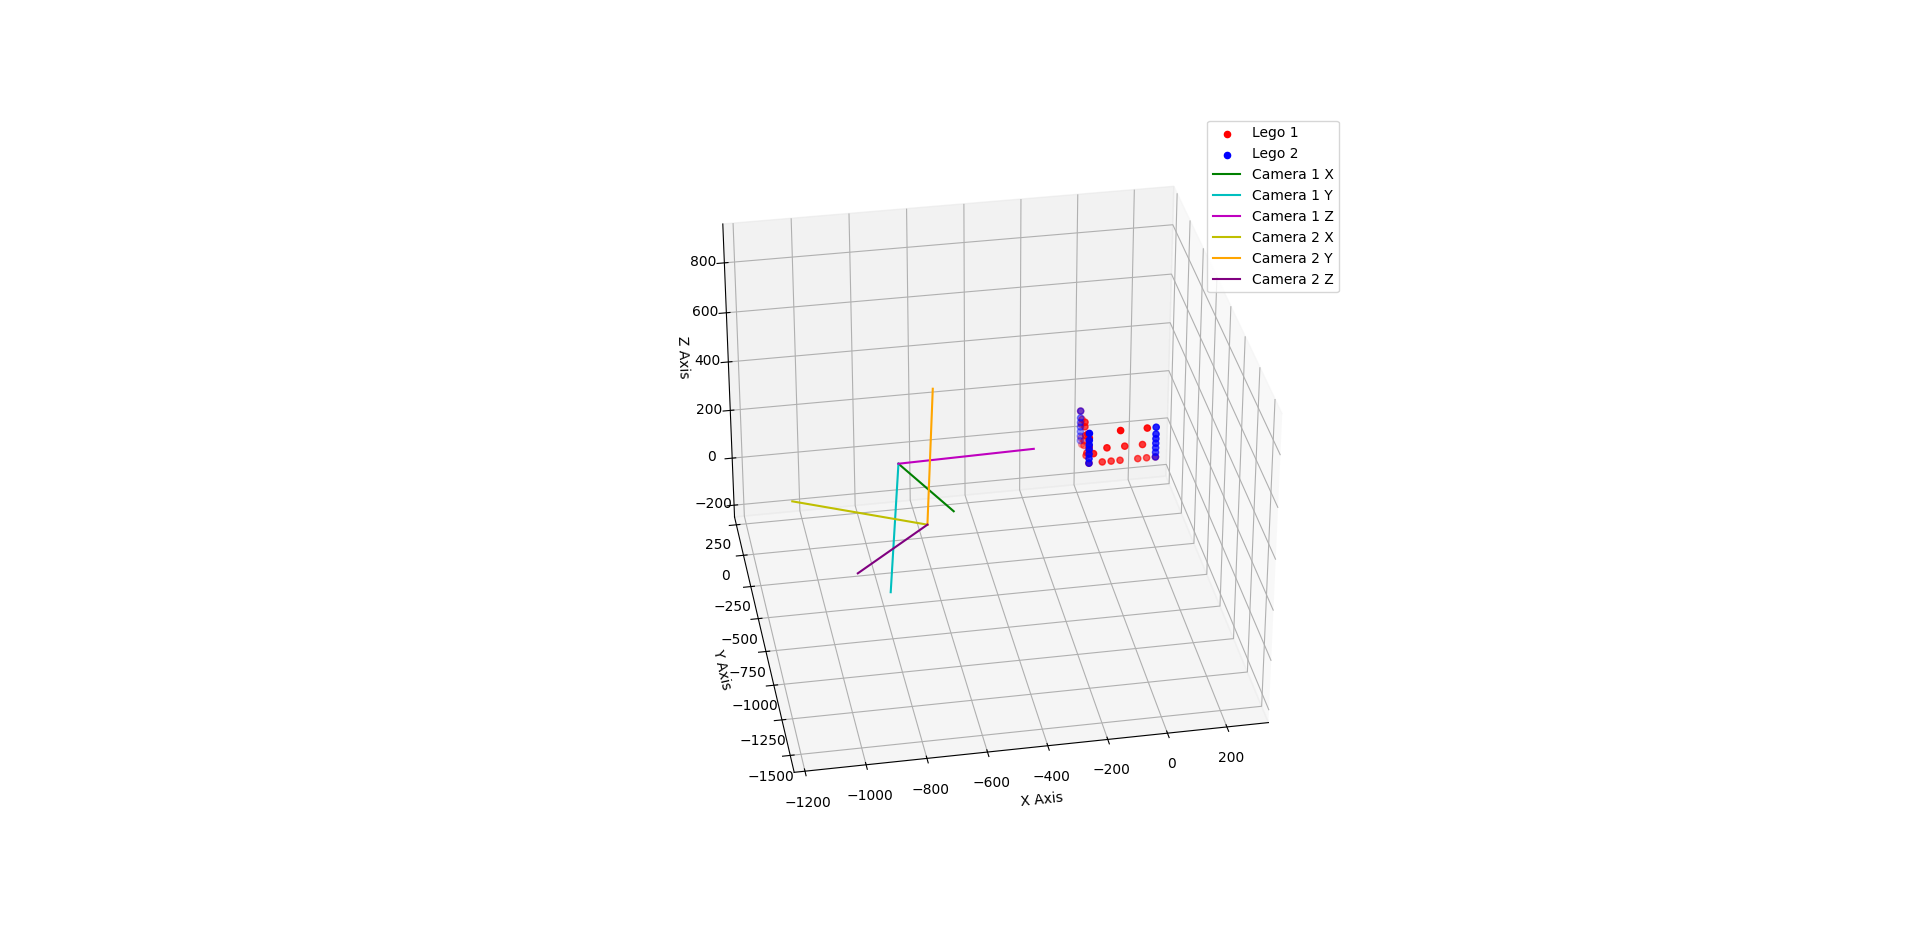
\includegraphics[width=\textwidth,  trim=350 0 350 0, clip]{Figure_3.png}
      \label{fig:image1}
  \end{minipage}\hfill
  \begin{minipage}{0.45\textwidth}
      \centering
      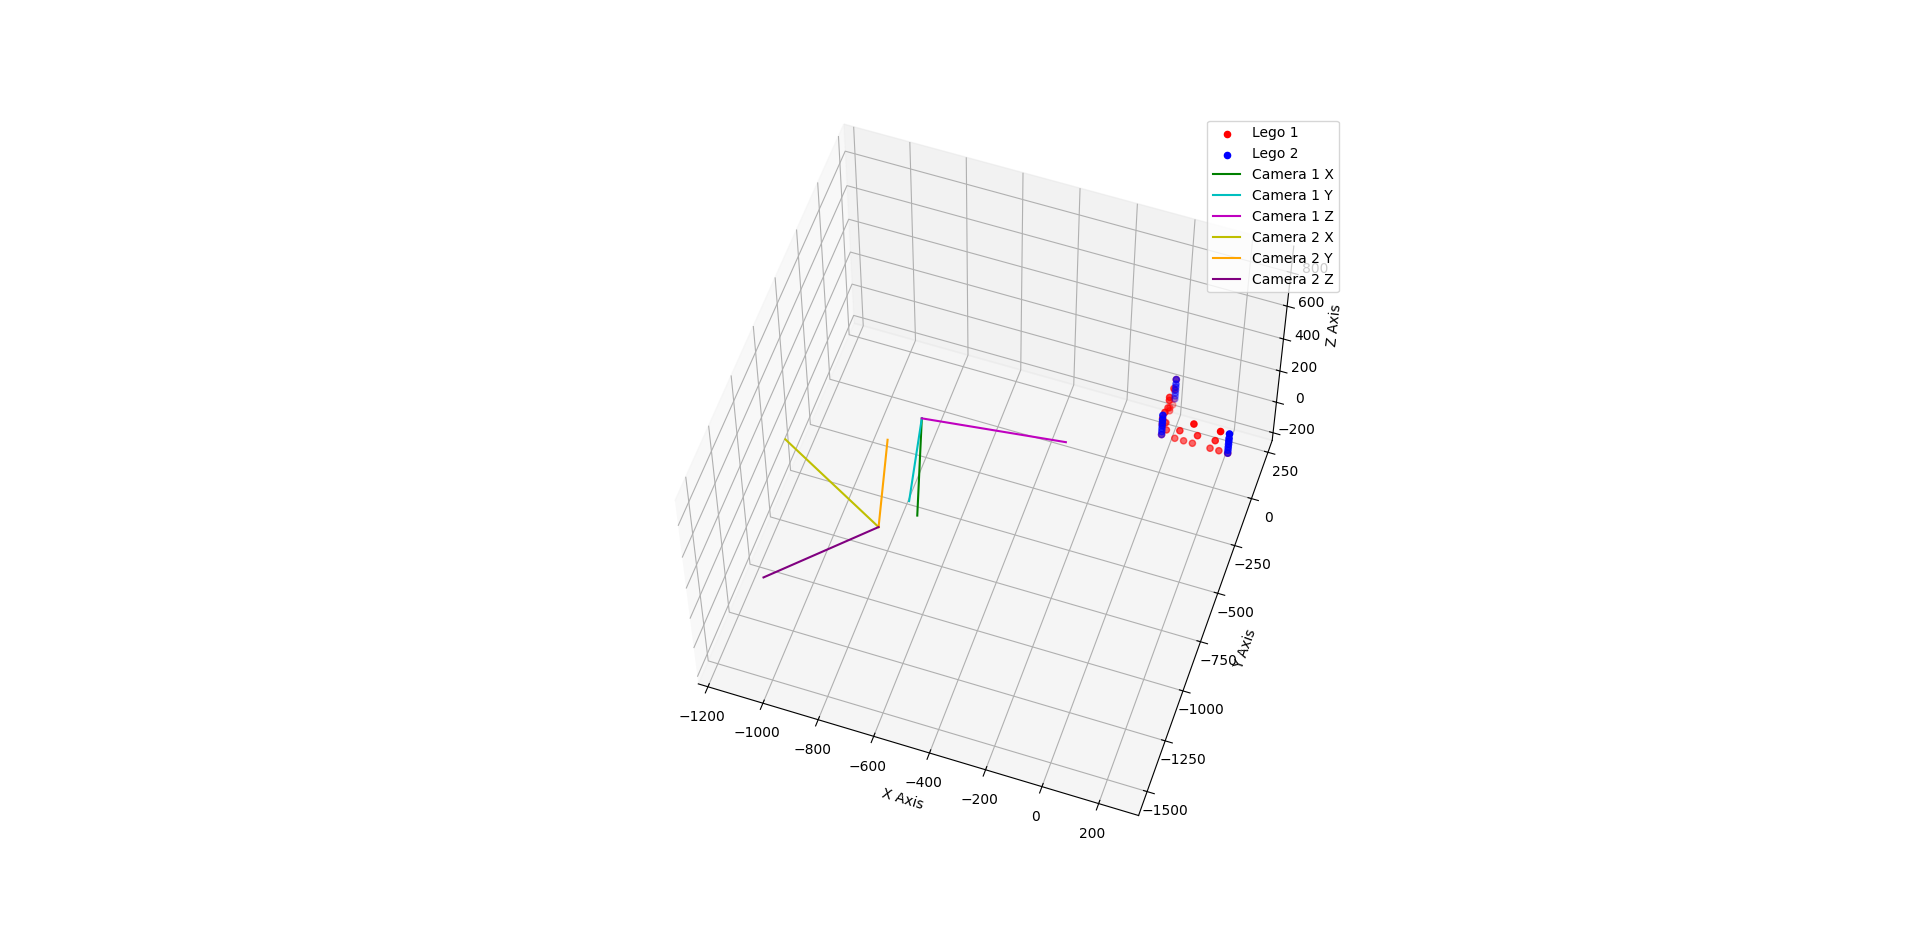
\includegraphics[width=\textwidth,  trim=350 0 350 0, clip]{Figure_4.png}
      \label{fig:image2}
  \end{minipage}
  \caption{Different views of 3D plot.}
  \label{fig:side_by_side}
\end{figure}

\textbf{Discussion:} \\
Discuss how the plot clarifies the relative positions and orientations of the cameras.

\newpage
\section{Problem 3: The Image of the World Coordinate System}
\textbf{Description:} \\
%Reference: https://engineering.purdue.edu/kak/computervision/ECE661Folder/Lecture19.pdf
%Prove that \(p_4\) is a homogeneous representation of the image of the world origin, and \(p_1, p_2, p_3\) are the images of the vanishing points of the world X, Y, and Z axes. Include mathematical derivations.

Let's express the $3 \times 4$ matrix $\mathbf{P}$ as
\[
\mathbf{P} = [\mathbf{p}_1 \; \mathbf{p}_2 \; \mathbf{p}_3 \; \mathbf{p}_4].
\]
Here, $\mathbf{p}_4$ is a homogeneous representation of the image of the world origin, and $\mathbf{p}_1$, $\mathbf{p}_2$, and $\mathbf{p}_3$ are the images of the vanishing points of the world $X$-, $Y$-, and $Z$-axes, respectively. Note that the ideal point along the world $x$-axis is given by
\[
[1 \; 0 \; 0 \; 0]^T.
\]
Since $\mathbf{P} \cdot [1 \; 0 \; 0 \; 0]^T = \mathbf{p}_1$, we have that the image of the ideal point is formed at the pixel whose homogeneous representation is $\mathbf{p}_1$. By the same reasoning, $\mathbf{p}_2$ is the image pixel for the ideal point along the $y$-axis, and $\mathbf{p}_3$ is the image pixel for the ideal point along the $z$-axis. The last column, $\mathbf{p}_4$, is the image of the world origin. The homogeneous representation of the world origin is
\[
[0 \; 0 \; 0 \; 1]^T.
\]
Its image is $\mathbf{P} \cdot [0 \; 0 \; 0 \; 1]^T = \mathbf{p}_4$.



\textbf{Results:} \\
% Demonstrate these statements using the two computed camera matrices. Include the plots of projected world axes overlaid on the images.
\begin{figure}[h]
  \centering
  \begin{minipage}{0.45\textwidth}
      \centering
      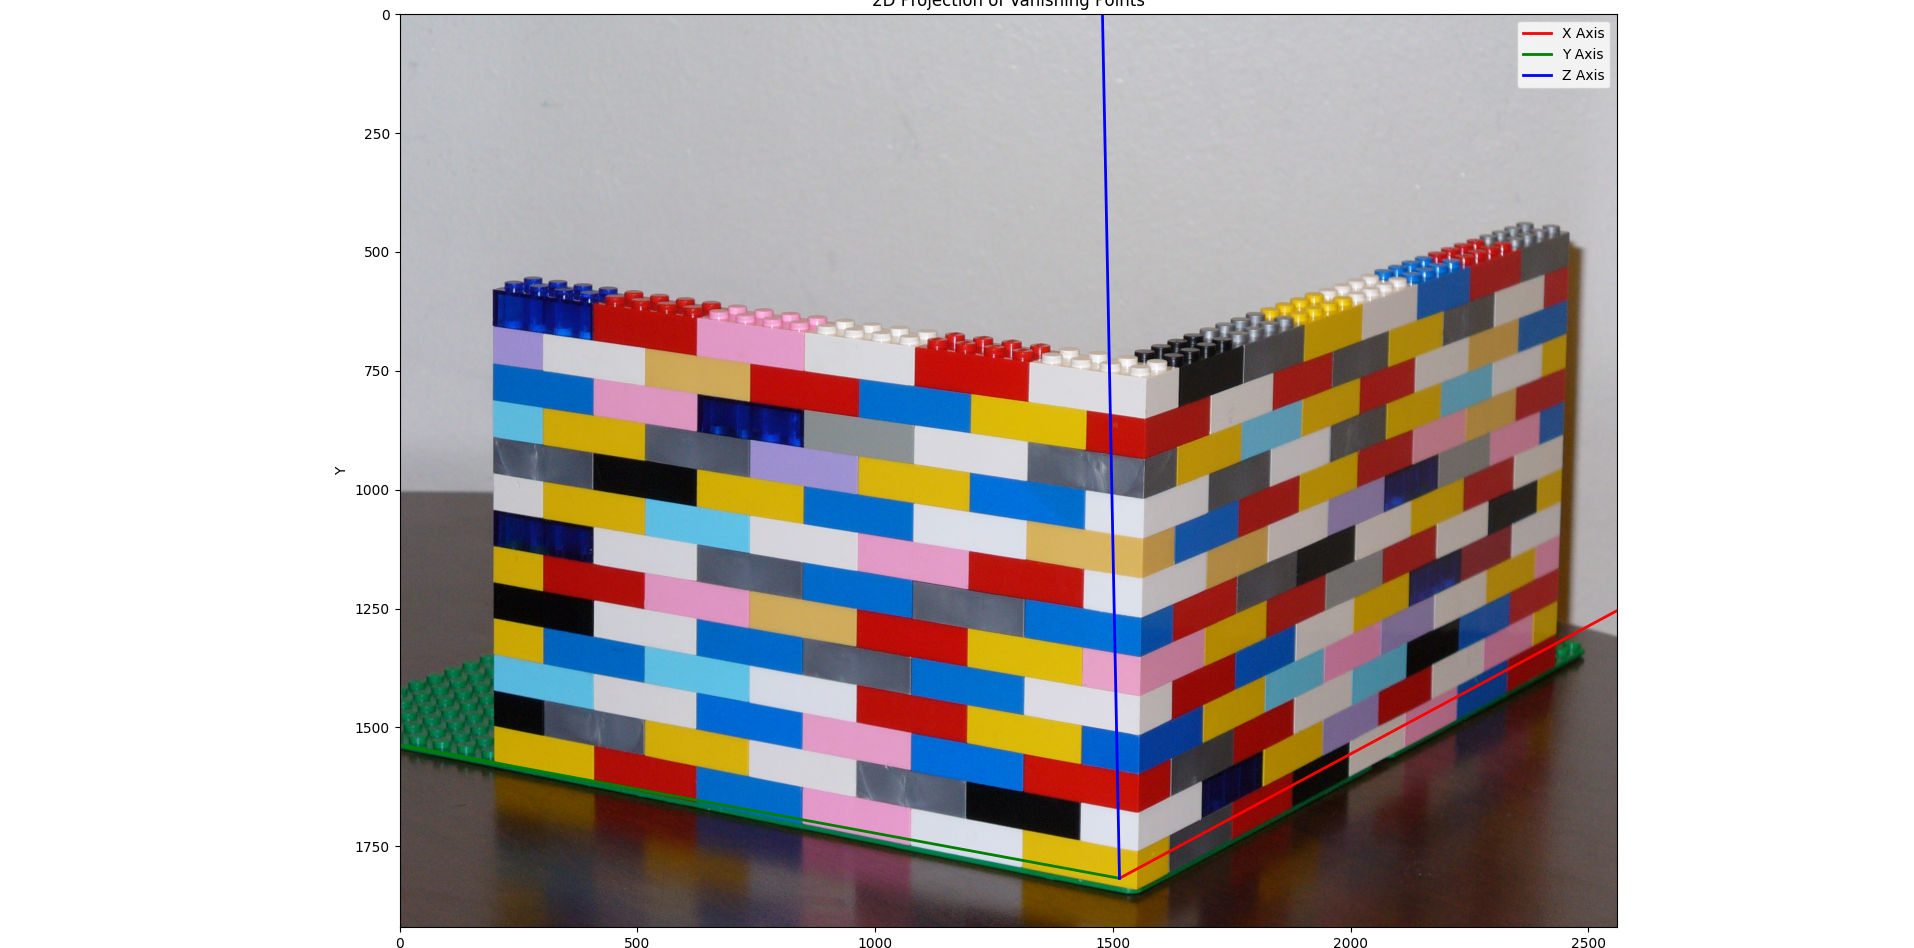
\includegraphics[width=\textwidth]{Figure_5.png}
      \caption{Projected world axes overlaid on lego 2.}
      \label{fig:image1}
  \end{minipage}\hfill
  \begin{minipage}{0.45\textwidth}
      \centering
      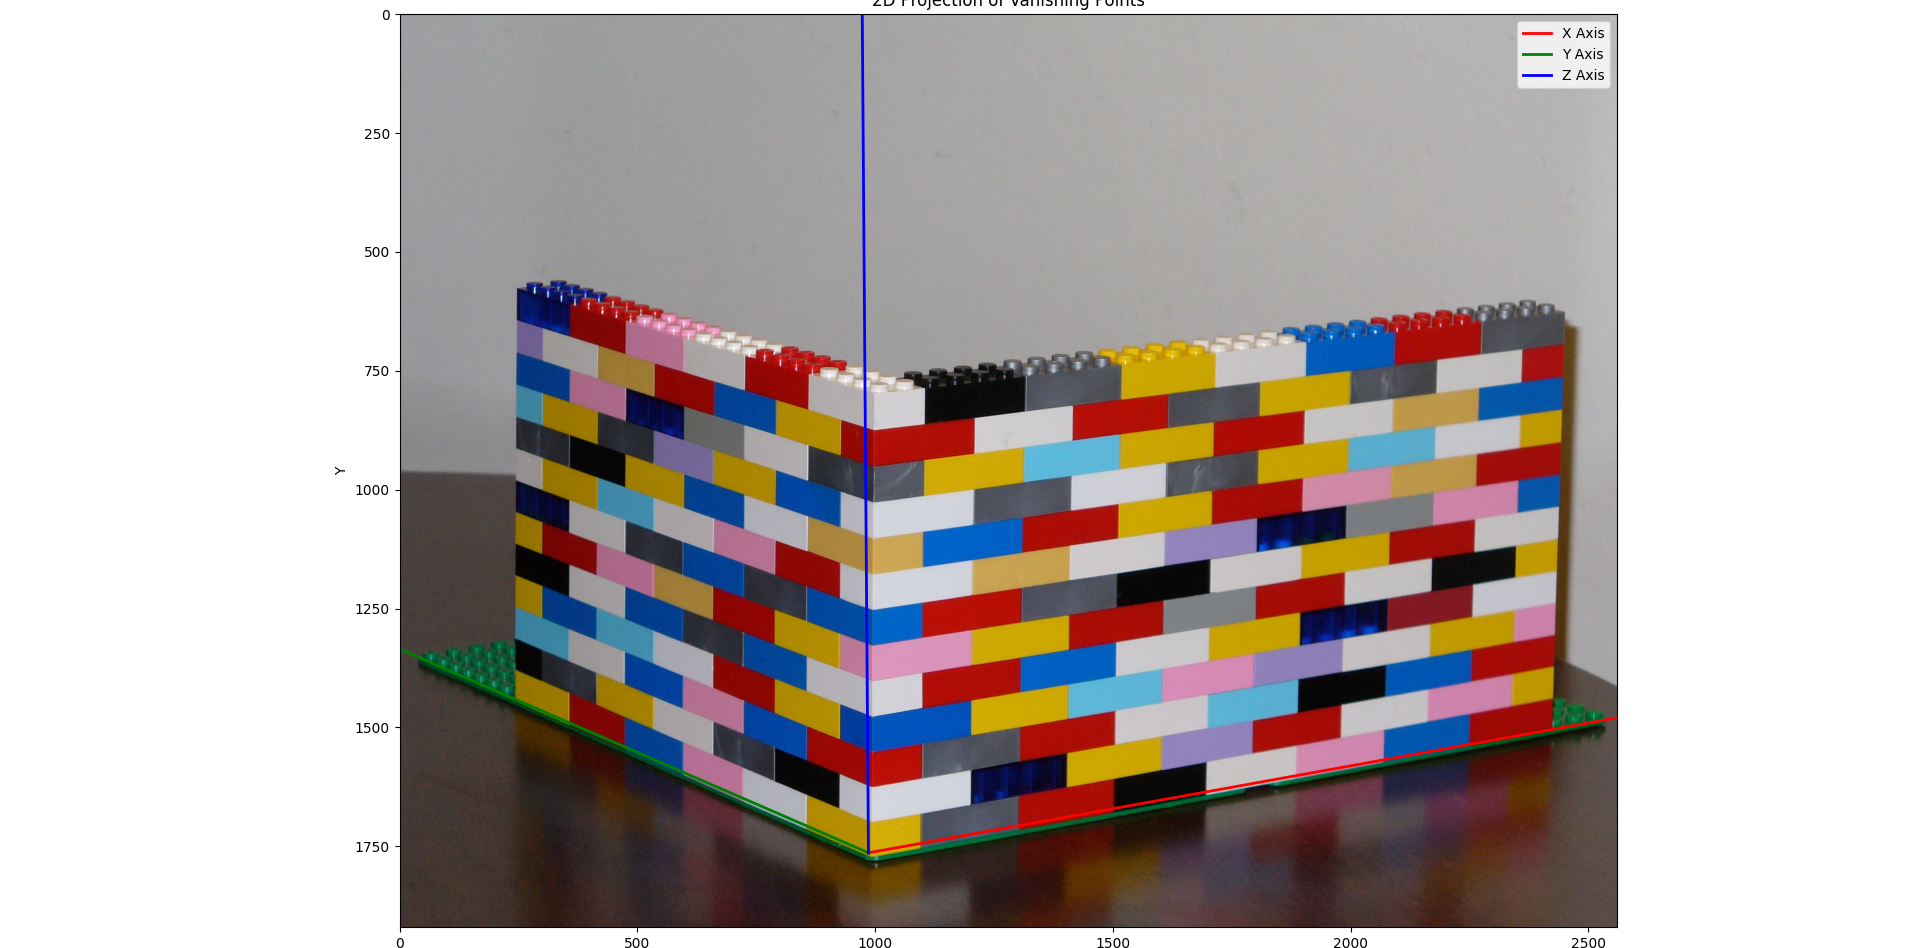
\includegraphics[width=\textwidth]{Figure_6.png}
      \caption{Projected world axes overlaid on lego 2.}
      \label{fig:image2}
  \end{minipage}
  \label{fig:side_by_side}
\end{figure}
\textbf{Discussion:} \\
Interpret the results and any observations.

\section{Problem 4: Epipolar Geometry}

\subsection{4a: Calculating Epipoles}
\textbf{Description:} \\
Describe the method used to calculate the epipoles \(e\) and \(e'\).

\textbf{Results:} \\
Provide the de-homogenized coordinates of both epipoles and discuss whether the coordinates make sense.

\subsection{4b: Computing the Fundamental Matrix and Epipolar Lines}
\textbf{Description:} \\
Explain how the fundamental matrix \(F\) was computed from \(P\) and \(P'\).

\textbf{Results:} \\
Display the epipolar lines on both images. Describe the visualization approach, including the use of color for corresponding lines.

\textbf{Discussion:} \\
Analyze the correctness of the epipolar lines and any observations on the correspondence between features.

\section{Conclusion}
Summarize the key findings of the report, including the results of the camera matrix calculations, decomposition, and epipolar geometry analysis.

\section{References}
List any references, textbooks, or online resources you used.

\end{document}
